\section{Introduction}
\label{sec:intro}
\subsection{Motivation}
The problem of reconstructing a signal (or image) from (possibly) nonlinear observations is widely encountered in standard signal acquisition and imaging systems. Our focus in this paper is the problem of signal reconstruction from \textit{modulo} measurements, where the modulo operation with respect to a positive real valued parameter $R$ returns the (fractional) remainder after division by $R$. See Fig.~\ref{fig:orgmodop} for an illustration.

%The problem of reconstructing the signal from its modulo measurements, referred as \textit{modulo recovery problem} in the literature, can be formalized as follows.

Formally, we consider a high dimensional signal (or image) $\mb{x}^* \in \R^n$. We are given modulo measurements of $\mb{x^*}$, that is, for each measurement vector $\mb{a_i} \in \R^n$, we observe:
\begin{equation}
y_i=\mod(\langle \mathbf{a_i} \cdot \mathbf{x^*} \rangle,R)~~~~\textnormal{for}~i = \{1,2,...,m\}, \nonumber
\label{eq:modmeas0}
\end{equation} 
The task is to recover $\mb{x^*}$ using the modulo measurements $\mb{y}$ and knowledge the measurement matrix $\mathbf{A} = \left[\mathbf{a_1~a_2~...~a_m}\right]^\t$. %Here, $\mod(\cdot)$ is modulo operation with respect to the period $R$. 

%\begin{figure}[h]
%	\begin{center}
%		\begin{tikzpicture}[scale=0.7, every node/.style={scale=0.7}]
%		\draw[<->] (-4,0) -- (4,0) node[right] {$t$};
%		\draw[->] (0,-1) -- (0,4) node[above] {$f(t)$};
%		\draw[scale=0.5, dashed, thick] (0,4)--(7,4) node[right]{$R$};
%		\draw (1.5,-0.5) node(below) {$p_i = 0$};
%		\draw (-1.5,-0.5) node(below) {$p_i = 1$};
%		\draw (0,-1.5) node(right) {$f(t) = \mod(t,R)$};
%		\draw[scale=0.5,domain=-7:0,smooth,variable=\x,blue,thick] plot ({\x},{\x+4});
%		\draw[scale=0.5,domain=0:7,smooth,variable=\x,blue, thick]  plot ({\x},{\x});
%		\end{tikzpicture}
%	\end{center}
%	\caption{\emph{Modified modulo function for the given problem}}
%	\label{fig:modop}
%\end{figure}

% One such example is the classical problem of phase retrieval, which arises in numerous imaging applications including ptychography, diffraction imaging and astronomical imaging \cite{shechtman2015phase, maiden2009improved}. In such imaging systems, due to the limitations of the optical sensors, only the magnitude of the light rays can be measured but not the phase. As each linear observation losses its phase, the effective forward model can be expressed as a composition of nonlinear absolute value function with the linear observation function. Though the phase retrieval problem is challenging ill-posed inverse problem, it is well-studied in the literature and there exists multiple provably efficient algorithmic procedures to solve it in different settings \cite{Netrapalli2013,candes2013phaselift,candes2015phase,wang2016sparse}.

This specific form of signal recovery is gaining rapid interest in recent times. Recently, the use of a novel imaging sensor that wraps the data in a periodical manner  has been shown to overcome certain hardware limitations of typical imaging systems \cite{Bhandari,Zhao2015}. Many image acquisition systems suffer from the problem of limited dynamic range; however, real-world signals can contain a large range of intensity levels, and if tuned incorrectly, most intensity levels can lie in the saturation region of the sensors, causing loss of information through signal clipping. The problem gets amplified in the case of multiplexed linear imaging systems (such as compressive cameras or coded aperture systems), where required dynamic range is very high because of the fact that each linear measurement is a weighted aggregation of the original image intensity values. 

\begin{figure}[!t]
	\begin{center}
		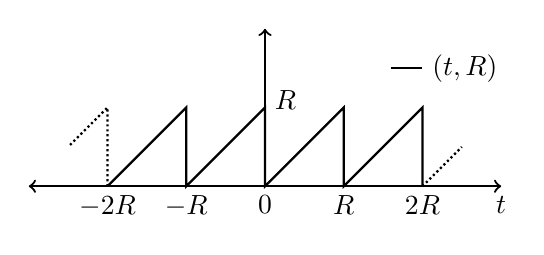
\begin{tikzpicture}
			\draw[<->,thick] (-3,0)--(3,0) node[anchor=north]{$t$};
			\draw (0,0) node[anchor=north]{$0$};
			\draw (0,1.1) node[anchor=west] {$R$};
			\draw (1,0) node[anchor=north]{$R$};
			\draw (2,0) node[anchor=north] {$2R$};
			\draw (-1,0) node[anchor=north]{$-R$};
			\draw (-2,0) node[anchor=north] {$-2R$};
			%\draw [densely dotted,thick] (-2.5,1)--(3,1);
			\draw[->,thick] (0,0)--(0,2);
			\draw[] (2,1.5) node[anchor=west] {{$\mod(t,R)$}};
			\draw[thick] (1.6,1.5) -- (2,1.5);
			\draw[thick] (-2,0) --(-1,1)-| (-1,0) -- (0,1) -| (0,0) --(1,1)-| (1,0) -- (2,1) -| (2,0);
			\draw[densely dotted,thick] (2,0)--(2.5,0.5);
			\draw[densely dotted,thick] (-2,0)|-(-2,1) -- (-2.5,0.5);
			\end{tikzpicture}
	\end{center}
	\caption{\emph{Modulo operation with respect to $R$}}
	\label{fig:orgmodop}
\end{figure}


The standard solution to this issue is to improve sensor dynamic range via enhanced hardware; this, of course, can be expensive. An intriguing alternative is to deploy special digital \emph{modulo} sensors. As the name suggests, such sensor wraps the observed signal intensity value around a given dynamic range parameter. This makes the forward model highly nonlinear and the reconstruction problem highly ill-posed. For most nonlinear ill-posed inverse problems, such results require overcomplete observations, meaning that the number of minimum measurements $m$ required for signal recovery is higher than the ambient dimension $n$ of the signal itself. For the cases where $m$ and $n$ are large, this requirement puts a heavy burden on computation and storage. 

In contrast, our focus is on solving the the inverse problem~\eqref{eq:modmeas0} with very few number of samples, {i.e.}, we are interested in the case $m<n$. While this makes the problem even more ill-posed, we show that such a barrier can be avoided if we assume that the underlying signal obeys a certain low-dimensional structure. We focus on the \emph{sparsity} assumption on the underlying signal, but our techniques could be extended to other signal structures.  

\subsection{Setup}
\label{subsec:setup}
The $\mod(\cdot,R)$ transfer function is many-to-one with infinite support. Thus, in this paper, we simplify our analysis by considering a simplified version of the modulo function that already inherits much of the challenging aspects of the original function. We consider a modified version that is truncated to only two periods of operation: one on the positive half and one in the negative half as shown in the Fig.~\ref{fig:compare}(a). %We also incorporate sparsity as a signal prior, thus capture the measurements in compressed sense, \textit{i.e.} $m<n$.
Assume $\mathcal{X} \subseteq \R^n$ to be a given (known) subset in the data space, and consider a signal (or image) $\mb{x}^* \in \mathcal{X}$. We construct $\mathbf{A} = \left[\mathbf{a_1~a_2~...~a_m}\right]^\t$ with i.i.d. Gaussian entries and $m<n$. We aim to recover the original signal $\mb{x^*}\in \R^n$ from its compressed modulo measurements $y_i$ defined as:
\begin{equation}
y_i=\mod(\langle \mathbf{a_i} \cdot \mathbf{x^*} \rangle,R)~\textnormal{for}~i = \{1,2,...,m\},
\label{eq:modmeas1}
\end{equation} 
where $\mod(\cdot)$ is modulo operation with respect to a fixed, real-valued parameter $R$. The primary assumption in our model is that the natural signal $\mathbf{x^*}$ is $s-$sparse in a chosen basis. 

%\begin{figure}[h]
%	\begin{center}
%		\begin{tikzpicture}[scale=0.7, every node/.style={scale=0.7}]
%		\draw[<->] (-4,0) -- (4,0) node[right] {$t$};
%		\draw[->] (0,-1) -- (0,4) node[above] {$f(t)$};
%		\draw[scale=0.5, dashed, thick] (0,4)--(7,4) node[right]{$R$};
%		\draw (1.5,-0.5) node(below) {$p_i = 0$};
%		\draw (-1.5,-0.5) node(below) {$p_i = 1$};
%		\draw (0,-1.5) node(right) {$f(t) = \mod(t,R)$};
%		\draw[scale=0.5,domain=-7:0,smooth,variable=\x,blue,thick] plot ({\x},{\x+4});
%		\draw[scale=0.5,domain=0:7,smooth,variable=\x,blue, thick]  plot ({\x},{\x});
%		\end{tikzpicture}
%	\end{center}
%	\caption{\emph{Modified modulo function for the given problem}}
%	\label{fig:modop}
%\end{figure}

\subsection{Our contributions}
In this paper, we propose a Alternating Minimization based recovery algorithm for exact reconstruction of signals from its compressed modulo measurements. We refer our algorithm as MoRAM- Modulo Recovery with Alternating Minimization. We also provide analytical proofs for exact recovery of signal using our algorithm. The key contribution of our approach is to identify and draw parallels between the problems of phase retrieval and modulo recovery, which allowed us to bring in the ideas from the classical phase retrieval solutions into relatively new setup of modulo recovery problems - which has been done for the first time to the best of our knowledge. 

The commonality that we identified in these two different class of problems is the need of undoing the effect of a piecewise linear function on the linear measurements in both the cases. While we deal with the modified version of modulo function with two periods in the case of modulo recovery, phase retrieval deals with absolute value function which is piece wise linear too. 

At the same time, difference between the behavior of both the functions is also evident, which restricts us from using the phase retrieval solutions as-is for solving modulo recovery problem. Fig.~\ref{fig:compare} compares both the modulo ($f(t)$) and absolute value ($g(t)$) functions. Both the functions are identical to identity function in the positive half, but differs significantly in the negative half. Absolute value function removes the sign from the negative input, thus it can be represented as a multiplicative process (multiplication with $-1$).  The modulo function adds the constant value $R$ in the negative inputs, thus can be represented as additive process (addition of $R$). Value of $p$ denotes whether the $R$ is added in the true measurement or not. It should be noted that the multiplication with $-1$ still preserves the magnitude information of the observations, while the additive process deforms the observation significantly, even more if the value of $R$ is higher. Additionally, the behavior of the modulo function is largely controlled by the value of the parameter $R$, while such parameter is non-existent in the case of absolute value function. 

Solving the phase retrieval problem is essentially equivalent to retrieving the phase value $ph_t$ corresponding to each measurement $t$. $ph_t$ can take only two values: $1$ if $t \geq 0$, or $-1$ if $t < 0$. On same lines, for modulo recovery case we introduce the term bin-index $p$, which acts similar to phase, and can take values $0$ if $t\geq 0$ or $1$ if $t<0$. It is understood that estimating the bin-index correctly leads to perfect recovery of the signal, and vice versa.
\begin{figure}[h]
	\begin{center}
		\begin{tabular}{cc}
			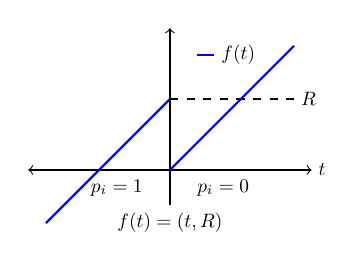
\begin{tikzpicture}[scale=0.45, every node/.style={scale=0.7}]
			\draw[<->] (-4,0) -- (4,0) node[right] {$t$};
			\draw[->] (0,-1) -- (0,4);
			\draw[scale=0.5, dashed, thick] (0,4)--(7,4) node[right]{$R$};
			\draw (1.5,-0.5) node(below) {$p_i = 0$};
			\draw (-1.5,-0.5) node(below) {$p_i = 1$};
			\draw[scale=0.5,blue,thick] (1.5,6.5)--(2.5,6.5) node[right,black]{$f(t)$};
			%\draw[scale=0.5,dotted,red,ultra thick] (1.5,5.5)--(2.5,5.5) node[right,black]{$g(t)$};
			\draw (0,-1.5) node(right) {$f(t) = \mod(t,R)$};
			\draw[scale=0.5,domain=-7:0,smooth,variable=\x,blue, thick] plot ({\x},{\x+4});
			\draw[scale=0.5,domain=0:7,smooth,variable=\x,blue, thick]  plot ({\x},{\x});
			%\draw[scale=0.5,domain=0:7,smooth,variable=\x,red, ultra thick, dotted]  plot ({\x},{\x});
			%\draw[scale=0.5,domain=-7:0,smooth,variable=\x,red, ultra thick, dotted]  plot ({\x},{-\x});
			\end{tikzpicture} &
			
			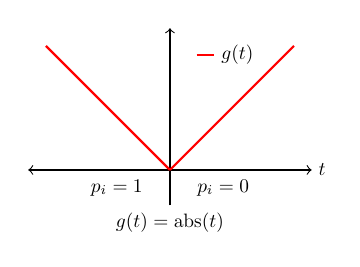
\begin{tikzpicture}[scale=0.45, every node/.style={scale=0.7}]
			\draw[<->] (-4,0) -- (4,0) node[right] {$t$};
			\draw[->] (0,-1) -- (0,4);
			%\draw[scale=0.5, dashed, thick] (0,4)--(7,4) node[right]{$R$};
			\draw (1.5,-0.5) node(below) {$p_i = 0$};
			\draw (-1.5,-0.5) node(below) {$p_i = 1$};
			%\draw[scale=0.5,blue,ultra thick] (1.5,6.5)--(2.5,6.5) node[right,black]{$f(t)$};
			\draw[scale=0.5,red,thick] (1.5,6.5)--(2.5,6.5) node[right,black]{$g(t)$};
			\draw (0,-1.5) node(right) {$g(t)=\mathrm{abs}(t)$};
			%\draw[scale=0.5,domain=-7:0,smooth,variable=\x,blue, ultra thick] plot ({\x},{\x+4});
			%\draw[scale=0.5,domain=0:7,smooth,variable=\x,blue, ultra thick]  plot ({\x},{\x});
			\draw[scale=0.5,domain=0:7,smooth,variable=\x,red,thick]  plot ({\x},{\x});
			\draw[scale=0.5,domain=-7:0,smooth,variable=\x,red, thick]  plot ({\x},{-\x});
			\end{tikzpicture} \\
			(a) & (b)
		\end{tabular}
	\end{center}
	\caption{\emph{Comparison between (a) absolute value function ($g(t) = \mathrm{abs}(t)$) ; and (b) modulo function ($f(t) = \mod(t,R)$)}}
	\label{fig:compare}
\end{figure}

We can measure the effect of such nonlinearity by analyzing the error between true measurements and observed measurements for the negative half of the number-line. In the case of phase retrieval problem, the error $e_a = \mathrm{abs}(t) - t = 2\mathrm{abs}(t),~\forall t <0$. Thus, the error (severity of the corruption) increases linearly with the magnitude of the true measurement. Measurements closer to zero are less affected compared to measurements far from zero. In standard phase retrieval setup, as the true measurements are linear combination of the samples from the Gaussian distribution, resulting distribution of the true measurements follows the Gaussian curve, which makes most of the true measurements concentrate close to zero; lowering the severity of the corruption.

For modulo recovery problem, the error is $e_m = \mod(t)-t = R,~\forall t<0$. Contrary to the case of phase retrieval, here the error is constant irrespective of magnitude of the true measurements. Even the true measurements lying very close to zero would experience the added error of $R$, and thus get severely affected. In the cases where $R$ is large, the magnitude of the additive corruption is way higher than the magnitude of the true measurement. Presence of such noise makes the recovery process very challenging.
\subsection{Techniques}

The proposed MoRAM algorithm is conceptually simple yet novel step in the direction of solving the problem of modulo recovery. Our work takes a fresh approach for solving the modulo recovery problem by borrowing the ideas from the well studied field of phase retrieval and compressive sensing. Our basic approach towards solving the modulo recovery problem is similar to the state-of-the-art phase retrieval approaches. As is the case with most of the non-convex algorithms, in the first step we identify a good initial guess $\mb{x^0}$ for our signal that lies relatively close to the true vector $\mb{x^*}$. The most commonly used initialization technique for phase retrieval is spectral initialization as described in \cite{Netrapalli2013}, but that doesn't work in our case due to variedly different behavior of modulo nonlinearity. We observe that the initialization is easier to obtain if we have access to rather a small number of true measurements than having a large number of modulo measurements (corrupted by nonlinearity). This leads us to a novel approach of recalculating the compressed measurements for the initialization. Having access to such corrected measurements, $\mb{x^0}$ can be calculated simply by using the first order estimator. Our method of recalculating the partial number of true measurements from the set of modulo measurements is intuitive yet gives provable guarantee for getting a initial vector significantly closer to the true signal. 

Our next challenge is to design a suitable algorithmic procedure that starts with the initial estimate and converge to the true signal. Again, we follow similar alternating minimization approach inspired from the phase retrieval solutions (\cite{Netrapalli2013}) that estimates the signal and the phase alternatively. To deal with the additive nature of the corruption, we introduce the Justice Pursuit based Alt-Min approach that leads to rapid convergence. Justice Pursuit is formulated specifically for compressive signal recovery in presence of unbounded sparse noise without requiring any parameter tuning. We also provide the theoretical analysis proving the convergence of the proposed algorithm. In particular,  we use the fact that justice pursuit algorithm manages to correct the corruption in bin-index values, provided the number of corrupted bin-indices is a fraction of total number of measurements. 

\subsection{Paper organization} 
The reminder of the paper is organized as follows. In section~\ref{sec:prior}, we briefly discuss the prior work. Sections~\ref{sec:prelim} contains notation and mathematical model used for our analysis. In section~\ref{sec:algo}, we introduce the MoRAM algorithm, and provide a theoretical analysis of its performance. We demonstrate the performance of our algorithm by providing series of numerical experiments in section~\ref{sec:exp}. Section~\ref{sec:disc} provides concluding remarks.